% !TEX root = main.tex

% TODO:
% REMARK:

\section{Data and Simulation samples}
\label{sec:DataAndMC}

	\subsection{Data sample}
	\label{ssec:DataAndMC_Data}

	% remember to mention golden json

	\subsection{Simulation sample}
	\label{ssec:DataAndMC_MC}

	\subsection{Correction on simulation sample}
	\label{ssec:DataAndMC_corMC}

		% pileup introduction is set on "vertex"
		\subsubsection{Pile-up Reweighing}
		\label{sssec:DataAndMC_PU}

			% https://twiki.cern.ch/twiki/bin/viewauth/CMS/PileupMCReweightingUtilities?fbclid=IwAR0SuZFQ5Um0IfZn1-CHXia6NPMYe2_7cz2OGXxhCYvNvfl_tTBke-w22l8

			As mention in section.\ref{ssec:PhysObj_pu}, pileup is the issue that bunch of vertices occuring at one collision. Although Monte Carlo sample may roughly cover the pileup interactions, the final distribution is also sensitive to the subtle content of primary vertex. Furthermore, the distribution of reconstructed vertices can be differently affected by the offline event selection cut and some high level trigger between real data and Monte Carlo sample. To fix the descrepancy between data and simulation, with any pileup number(number of primary vertices) bin, we compare the data and MC distribution and get the data/MC value bin by bin. The gotten scale factors under pileup number bins will be applied on the analyzed MC to correct the weight of each event.

		\subsubsection{Jet Energy correction, smearing and resolution}
		\label{sssec:DataAndMC_JE_CSR}

			The JEC and JER are mentioned in section.\ref{ssec:PhysObj_jet} previously.

		\subsubsection{Lepton efficiency Scale Factor}
		\label{sssec:DataAndMC_LepEffSF}

		With selection cut or quality pick-up on physics objects like leptons, there must be difference in the selection performance between data and MC. To correct the discrepancy, the often method is apply a scale factor on the $p_T$-$\eta$ space to correct the weight of this event. The scale factor S.F. is calculated from selection efficiency performance of known data and MC by Eq.\ref{eq:eff_SF}. 

		\begin{equation}
		S.F. = \frac{\epsilon_{data}(p_T,\eta)}{\epsilon_{MC}(p_T,\eta)}
		\label{eq:eff_SF}
		\end{equation}

		It is usually implemented by tag-and-probe method\cite{tagandprobe_twiki}. There are efficiency S.F. of muonISO, muonID, muonTrigger, ElectronReco, ElectronID, and ElectronTrigger necessary to be considered. The gotten scale factors under $p_T$-$\eta$ space are shown below:

		\begin{figure}[H]
			\centering
			    \subfigure[Muon ISO]{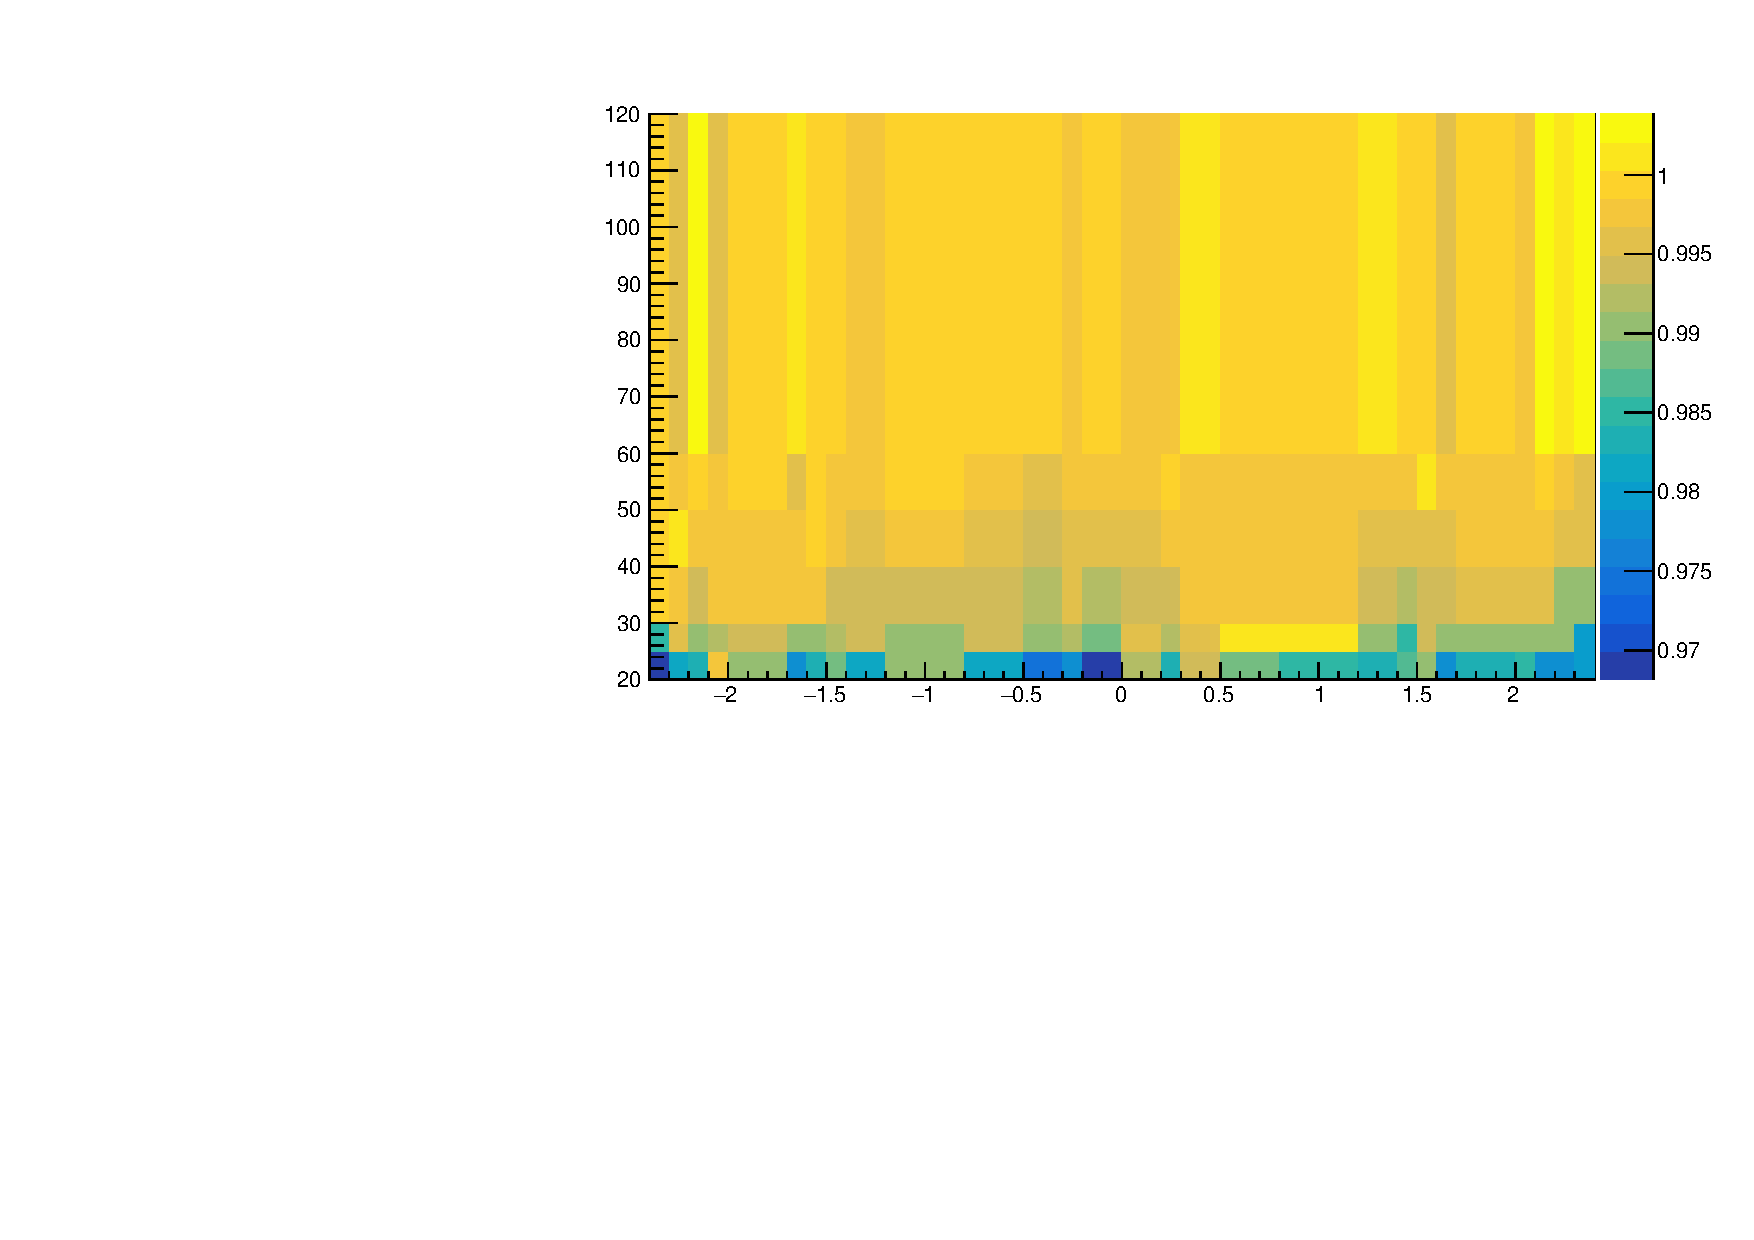
\includegraphics[width=0.32\textwidth]{Figures/DataMC/mu_ISO.pdf}}
			    \subfigure[Muon ID]{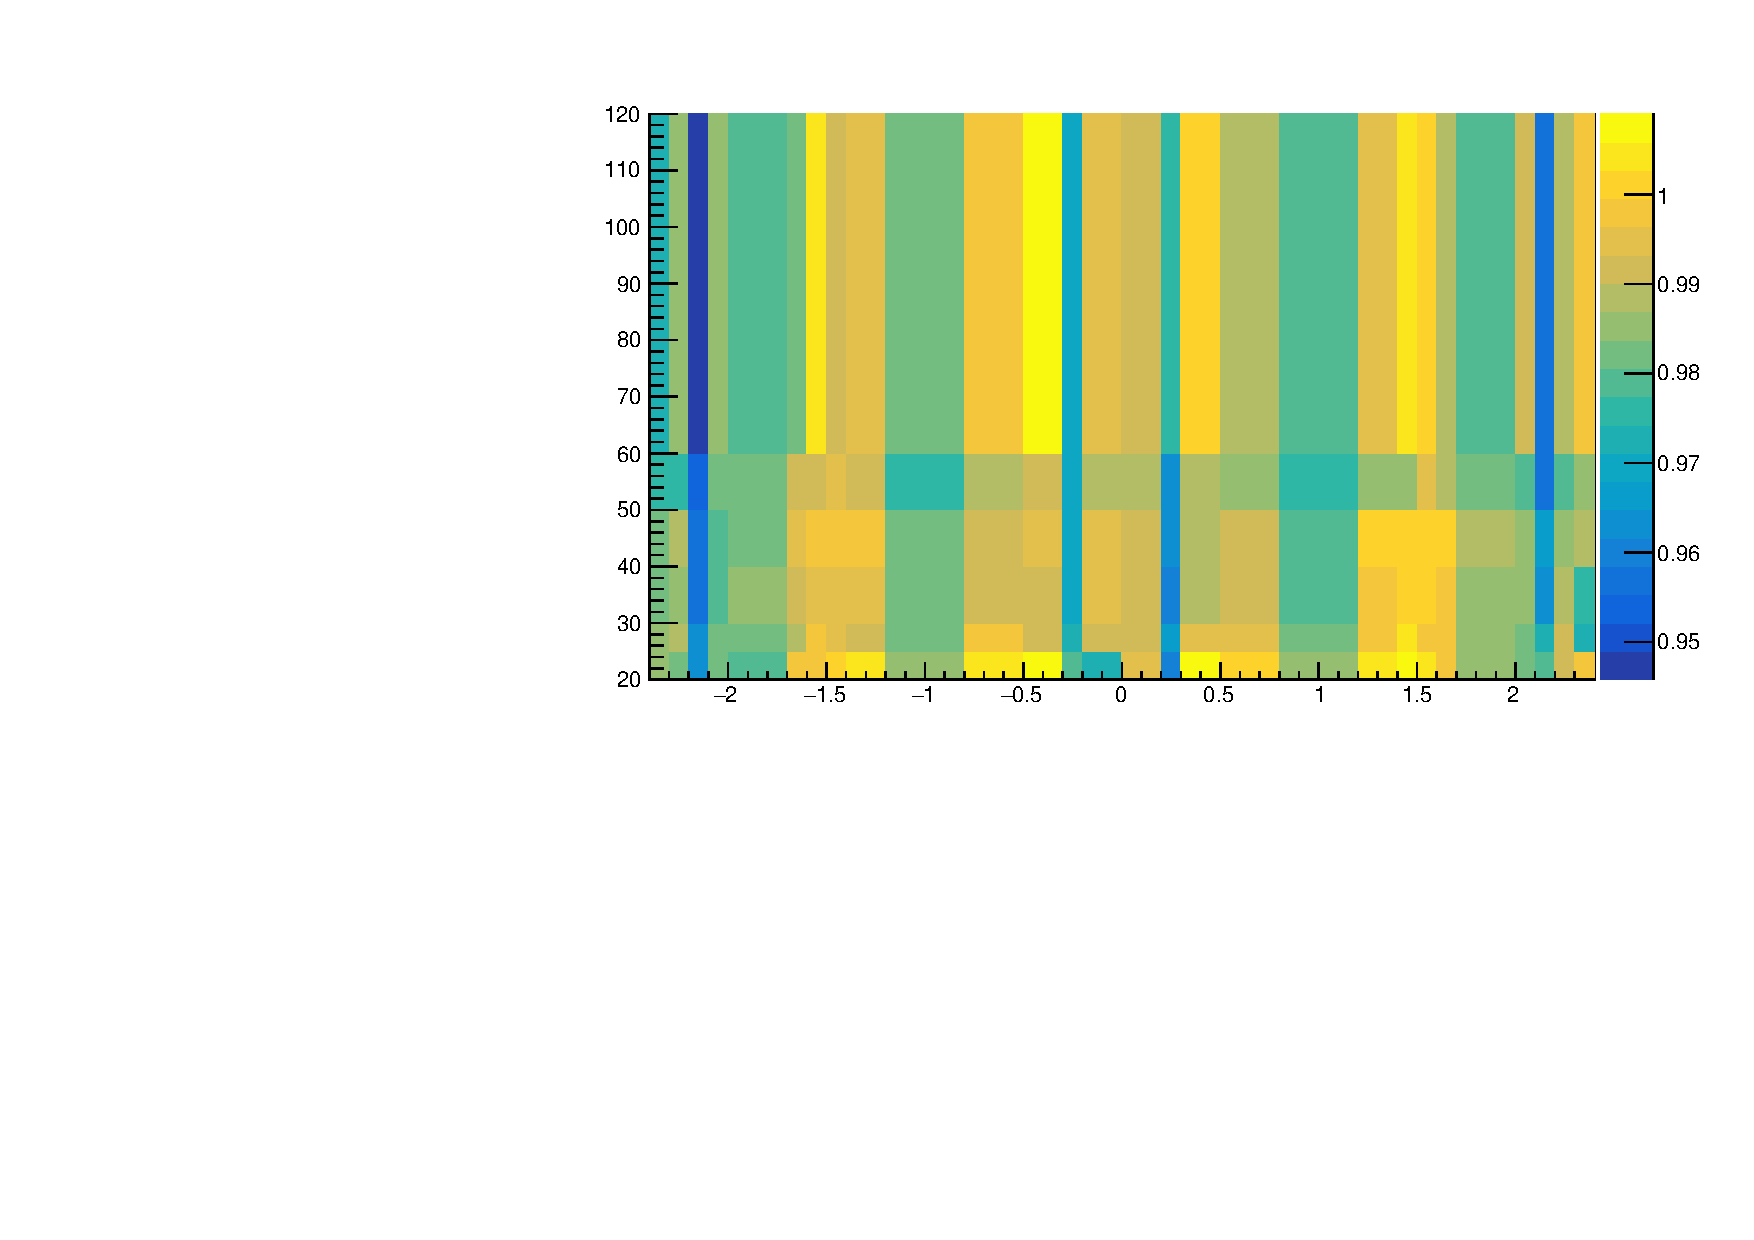
\includegraphics[width=0.32\textwidth]{Figures/DataMC/mu_ID.pdf}}
			    \subfigure[Muon High Level Trigger]{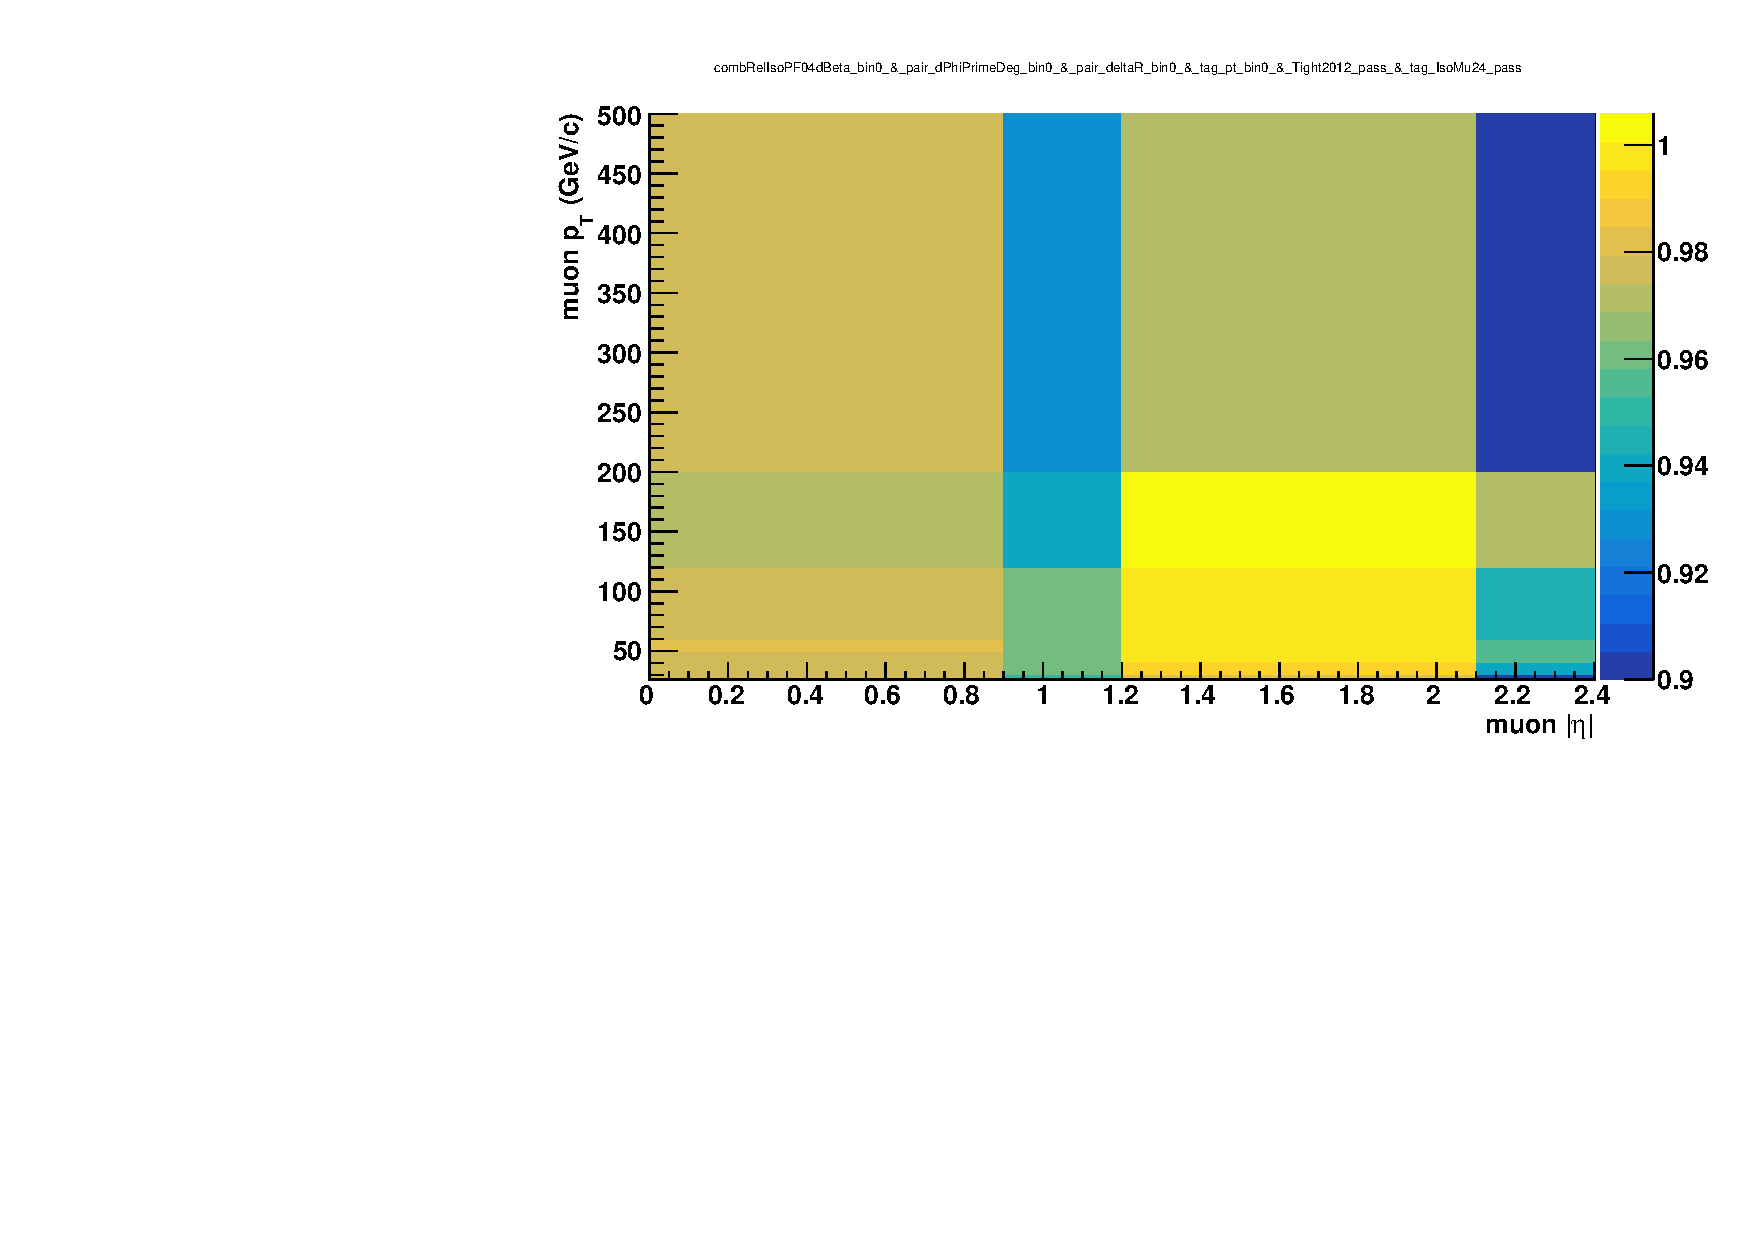
\includegraphics[width=0.32\textwidth]{Figures/DataMC/mu_Trg.pdf}}\\
			\end{figure}{}
			\FloatBarrier
			\begin{figure}[H]
			\centering
			    \subfigure[Electron Reco]{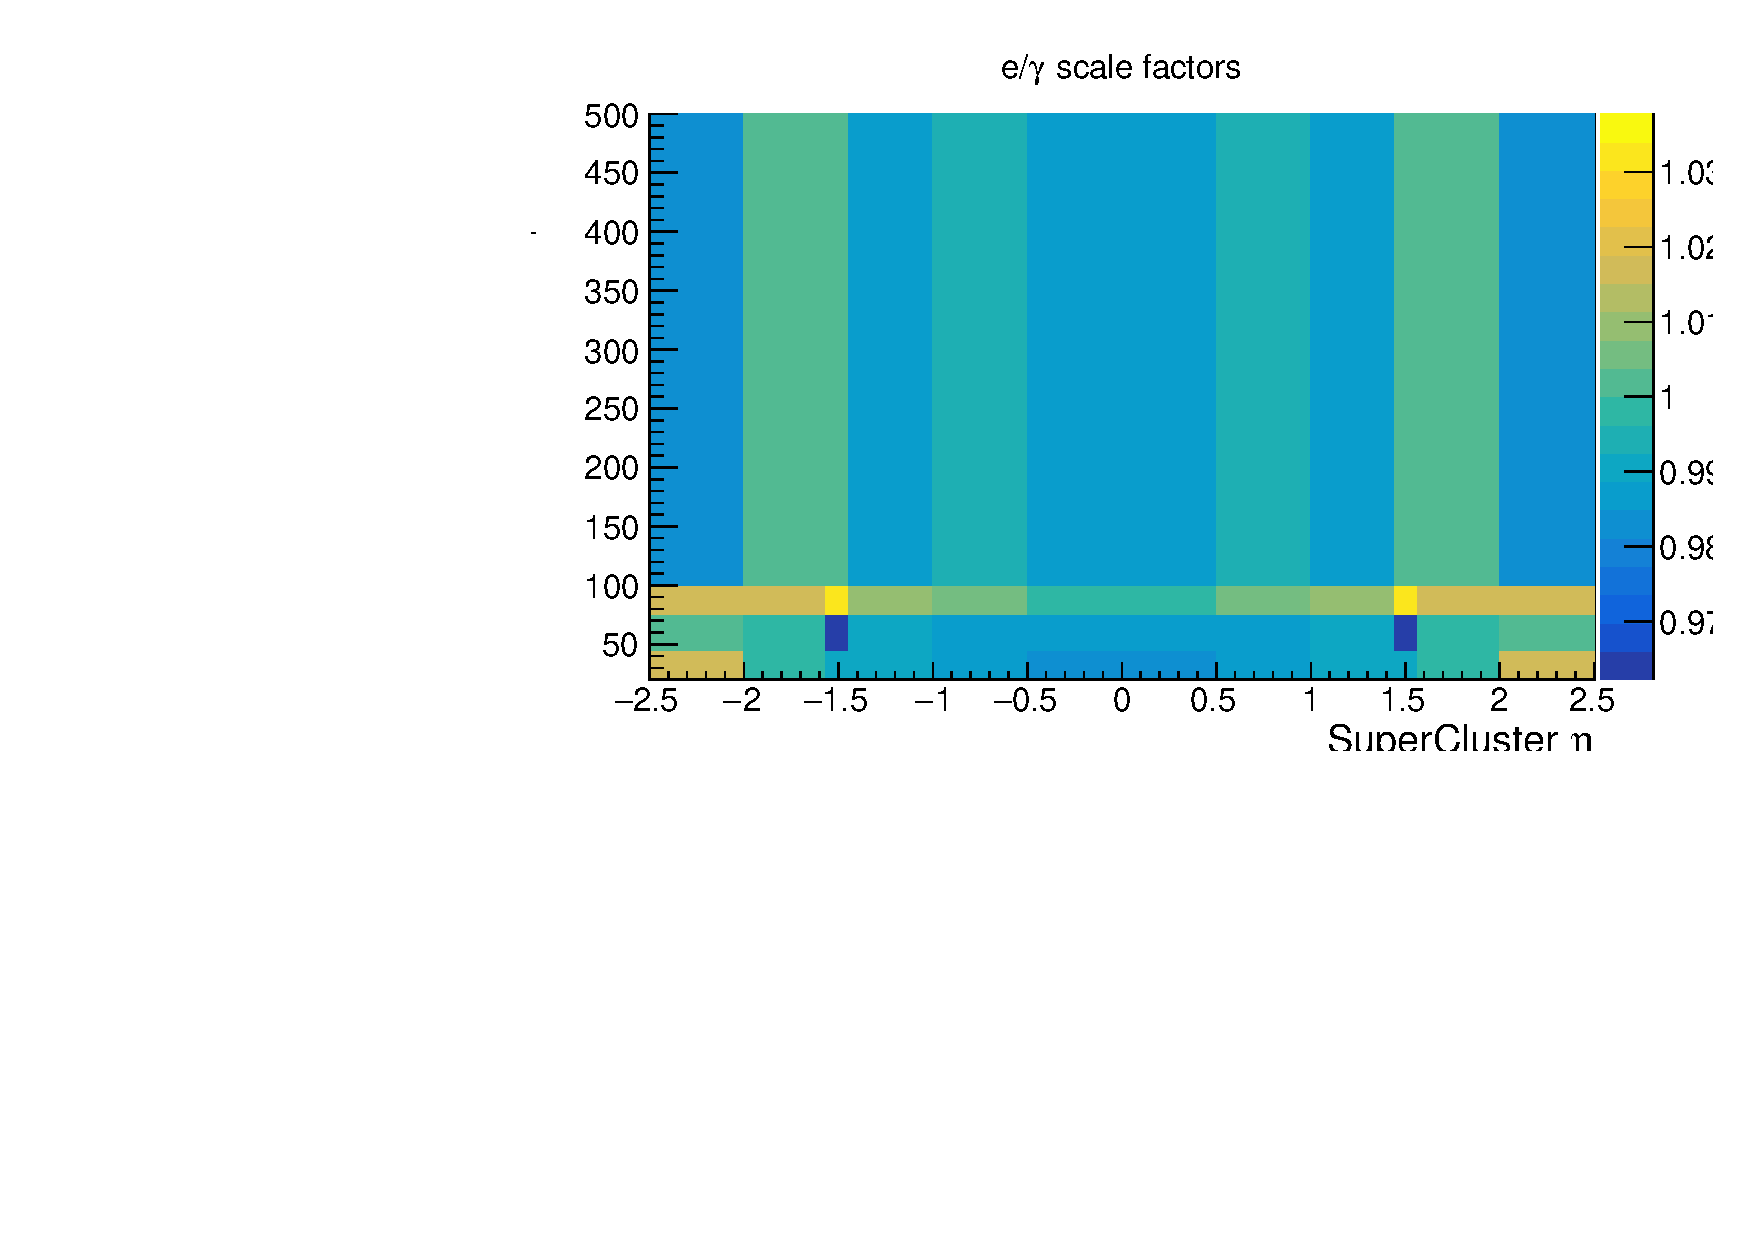
\includegraphics[width=0.32\textwidth]{Figures/DataMC/el_Reco.pdf}}
			    \subfigure[Electron ID]{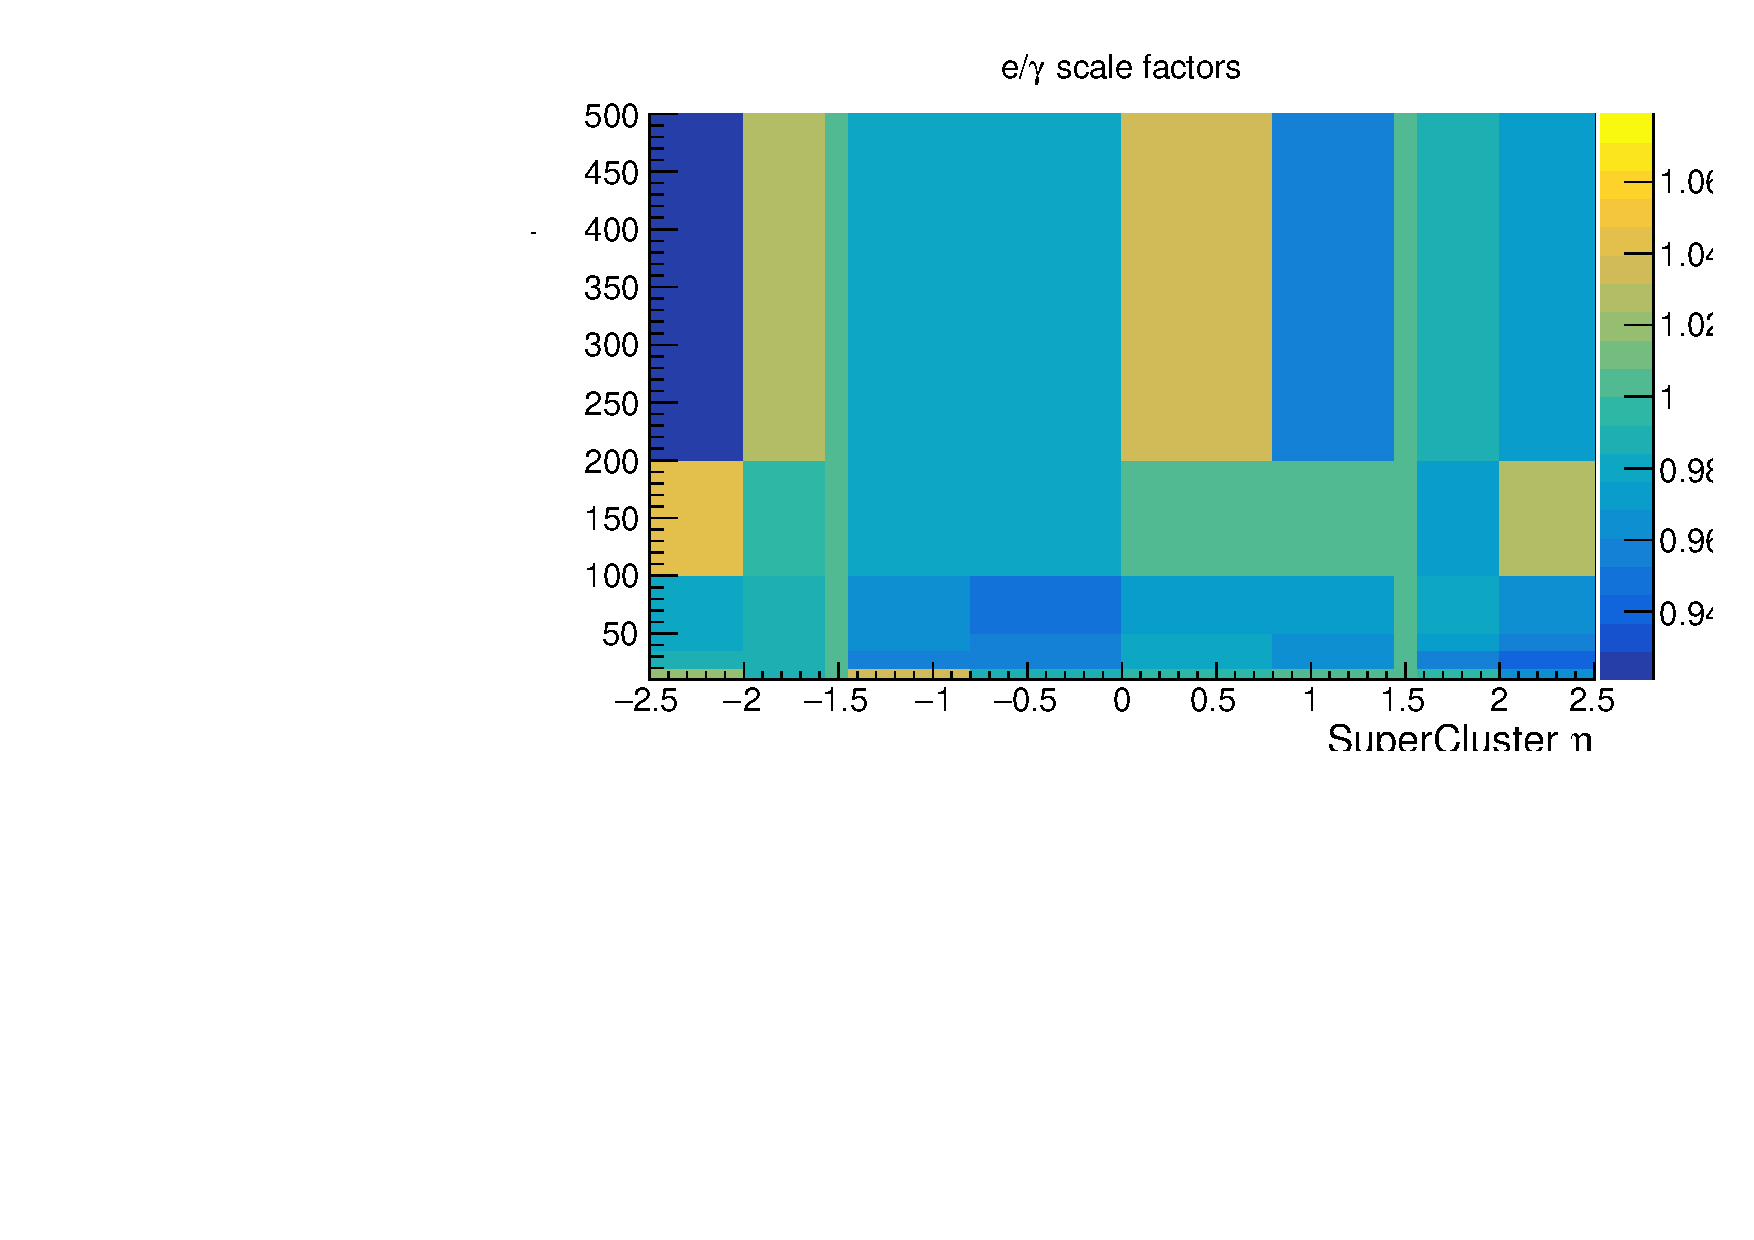
\includegraphics[width=0.32\textwidth]{Figures/DataMC/el_ID.pdf}}
			    \subfigure[Electron High Level Trigger]{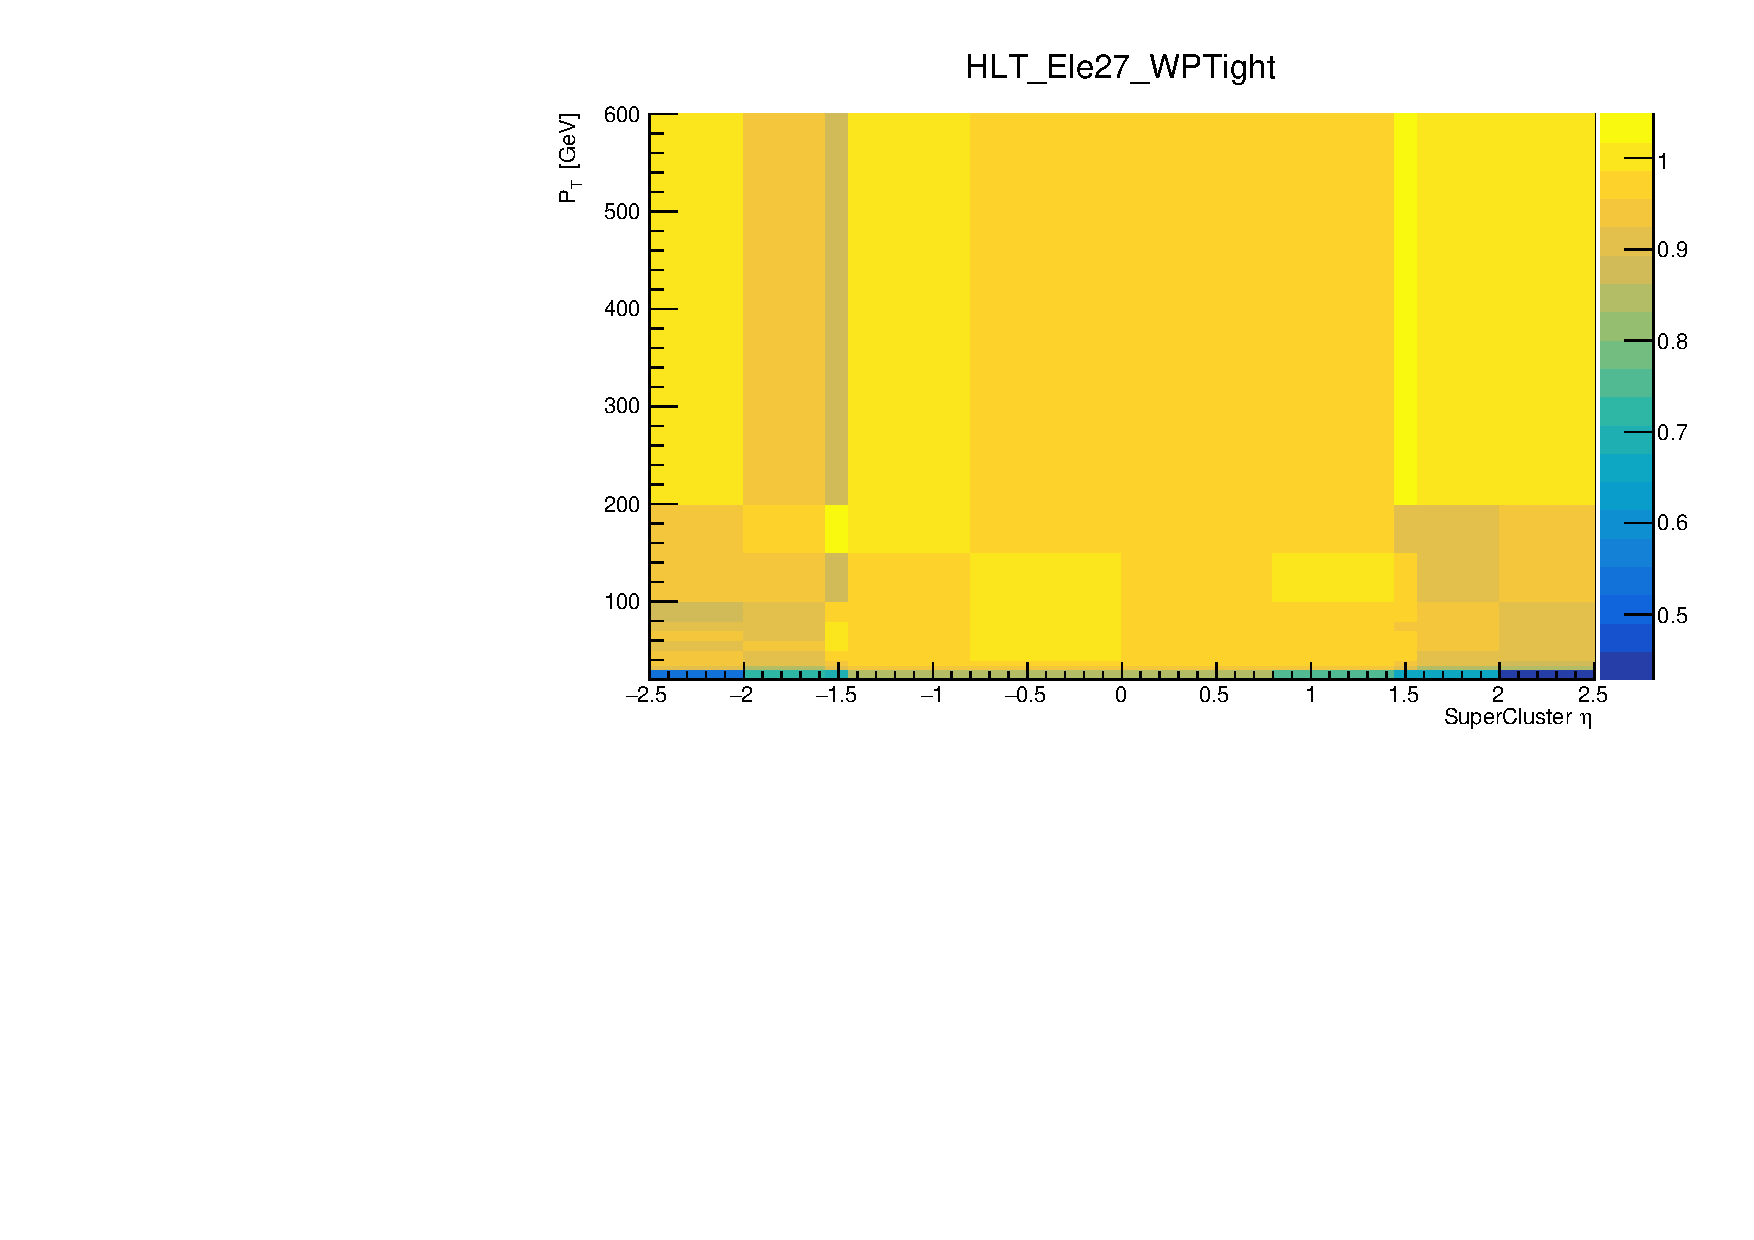
\includegraphics[width=0.32\textwidth]{Figures/DataMC/el_Trg.pdf}}\\
			   \caption{Lepton efficiency scale factor (x-axis:$\eta$, y-axis:$p_T$)}
			\label{DataMC:fig:lepsf}
			\end{figure}
			\FloatBarrier

		\subsubsection{b-tagging Reweighing}
		\label{sssec:DataAndMC_btagSF}

			The b-tagging reweight have to obtained by b-tagging scale factors and the b-tagging efficiency under b/c/light(udsg)-flavor identification.(The b-tagging efficiency means the ratio of jets which should pass b-tagging and really pass b-tagging) The b-tagging scale factor complies with the same concept as efficiency scale factor. Because of applying the selection which is deepCSV cut (DeepCSV Medium and DeepCSV Loose), data and MC have different performance on selection efficiency, then the S.F. of b-tagging is still got with Eq.\ref{eq:eff_SF} by BTV POG\cite{btvpog_twiki} with full RunII data. However, the reweight on each event is not just about scale factor. Since we apply the b-tagging tool on any jets which pass the jet-selection(Table.\ref{PhysObj:tb:sel_jet}), all the tagged jets and non-tagged jets should be considered to have influence about the b-tagging efficiency difference and to affect the event weight \cite{btagreweight_twiki}. The eventual formula of b-tagging event reweighting is derived by data correct tagged probability($P(data)$) divided by MC's($P(MC)$) (Eq.\ref{eq:btag_weight_1}). Both probabilities are calculated by Eq.\ref{eq:btag_weight_2} reasonabliy. 

			\begin{equation}
			weight = \frac{P(data)}{P(MC)}
			\label{eq:btag_weight_1}
			\end{equation}

			\begin{equation}
			\begin{split}
			P(MC) = \prod_{i=tagged} \epsilon_i(p_T,\eta) \prod_{j=non-tagged} (1-\epsilon_j(p_T,\eta)) \;\;\;\;\;\;\;\;\;\;\;\;\;\;\; \\
			P(data) = \prod_{i=tagged} SF(p_T,\eta) \cdot \epsilon_i(p_T,\eta) \prod_{j=non-tagged} (1- SF(p_T,\eta) \cdot \epsilon_j(p_T,\eta))
			\label{eq:btag_weight_2}
			\end{split}
			\end{equation}

			As mentioned previously, the S.F. are obtained, and b-tagging efficiency of three types of flavor jets are gotten by hand with simulated $t\bar{t}$ sample (Fig.\ref{DataMC:fig:tt_eff_btag}). Also, the b-tagging efficiency of three flavor jets are obviously different and they are calculated on the $p_T$-$\eta$ space.

			\begin{figure}[H]
			\centering
			    \subfigure[b]{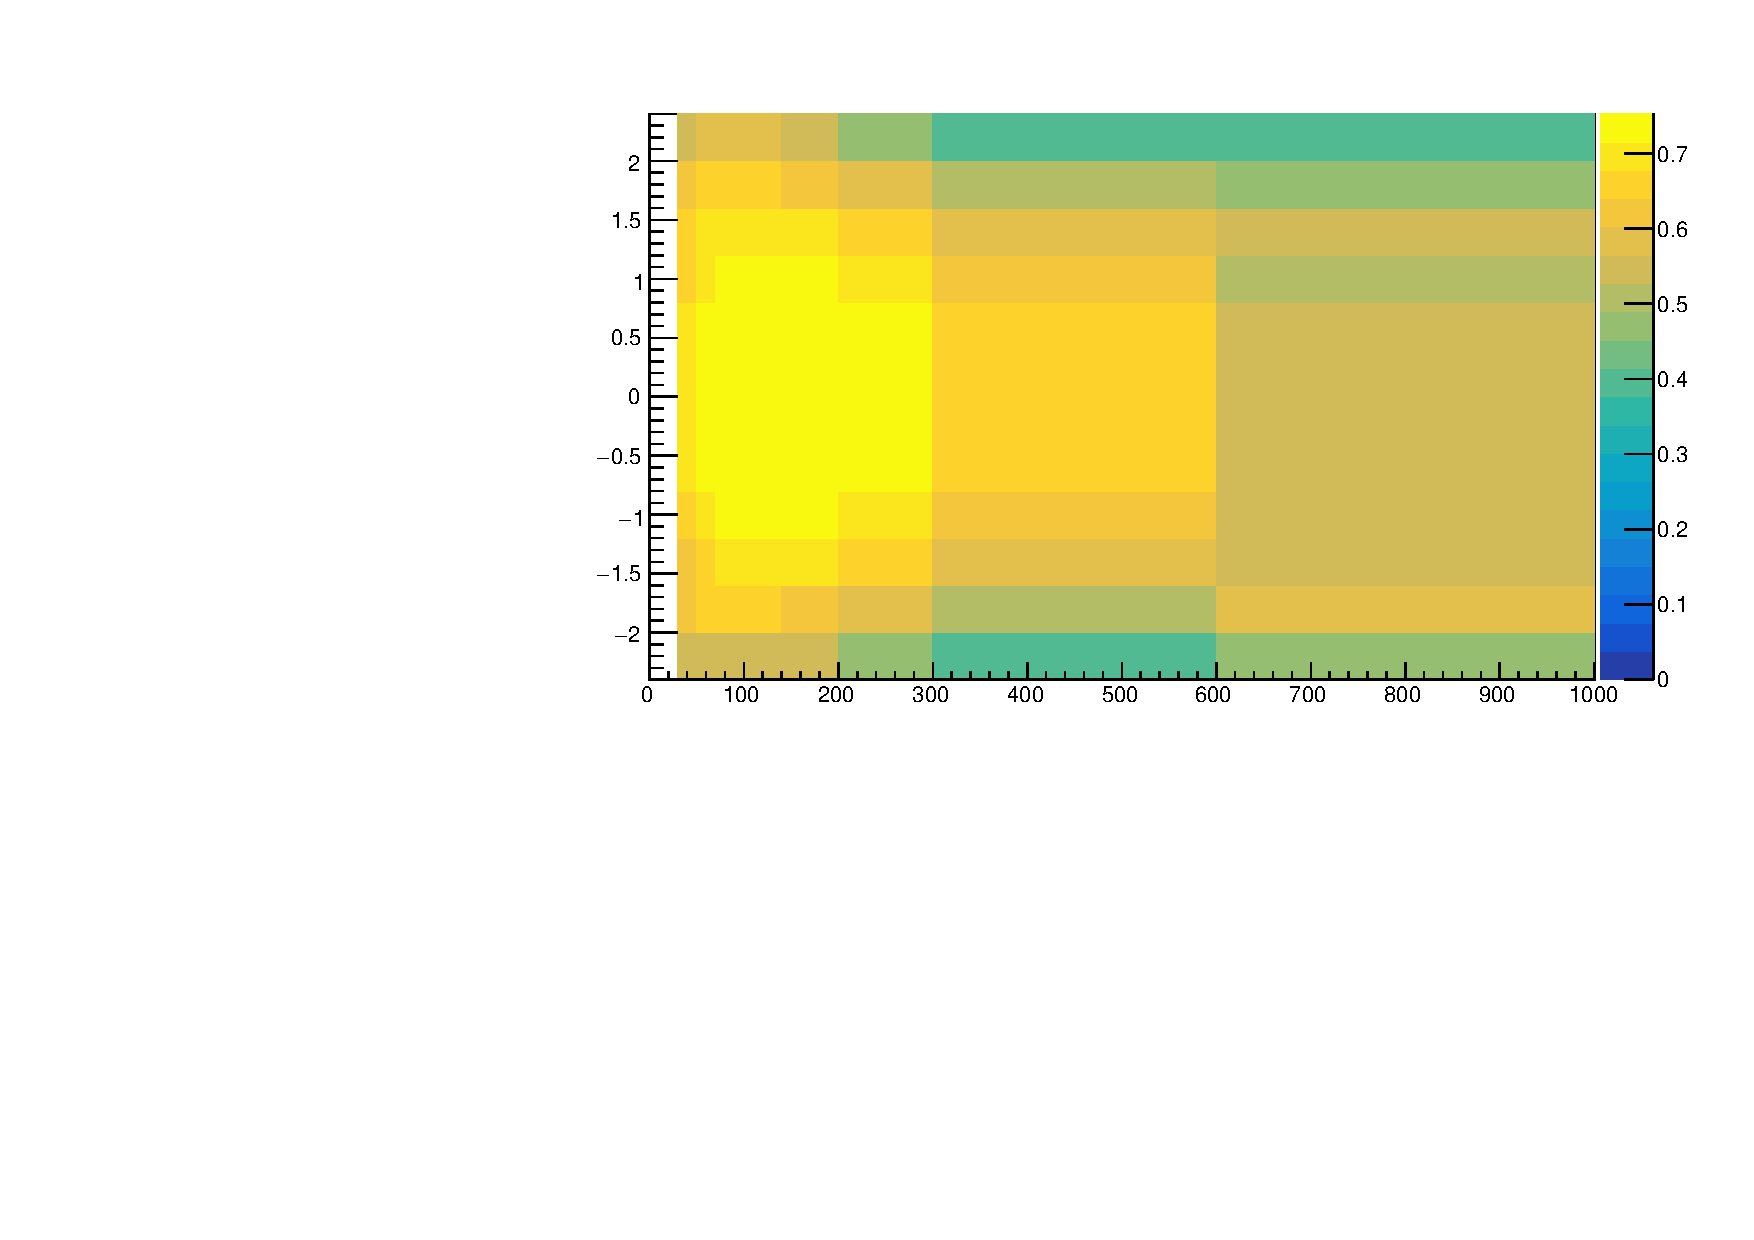
\includegraphics[width=0.45\textwidth]{Figures/DataMC/tt_eff_b.pdf}}
			    \subfigure[c]{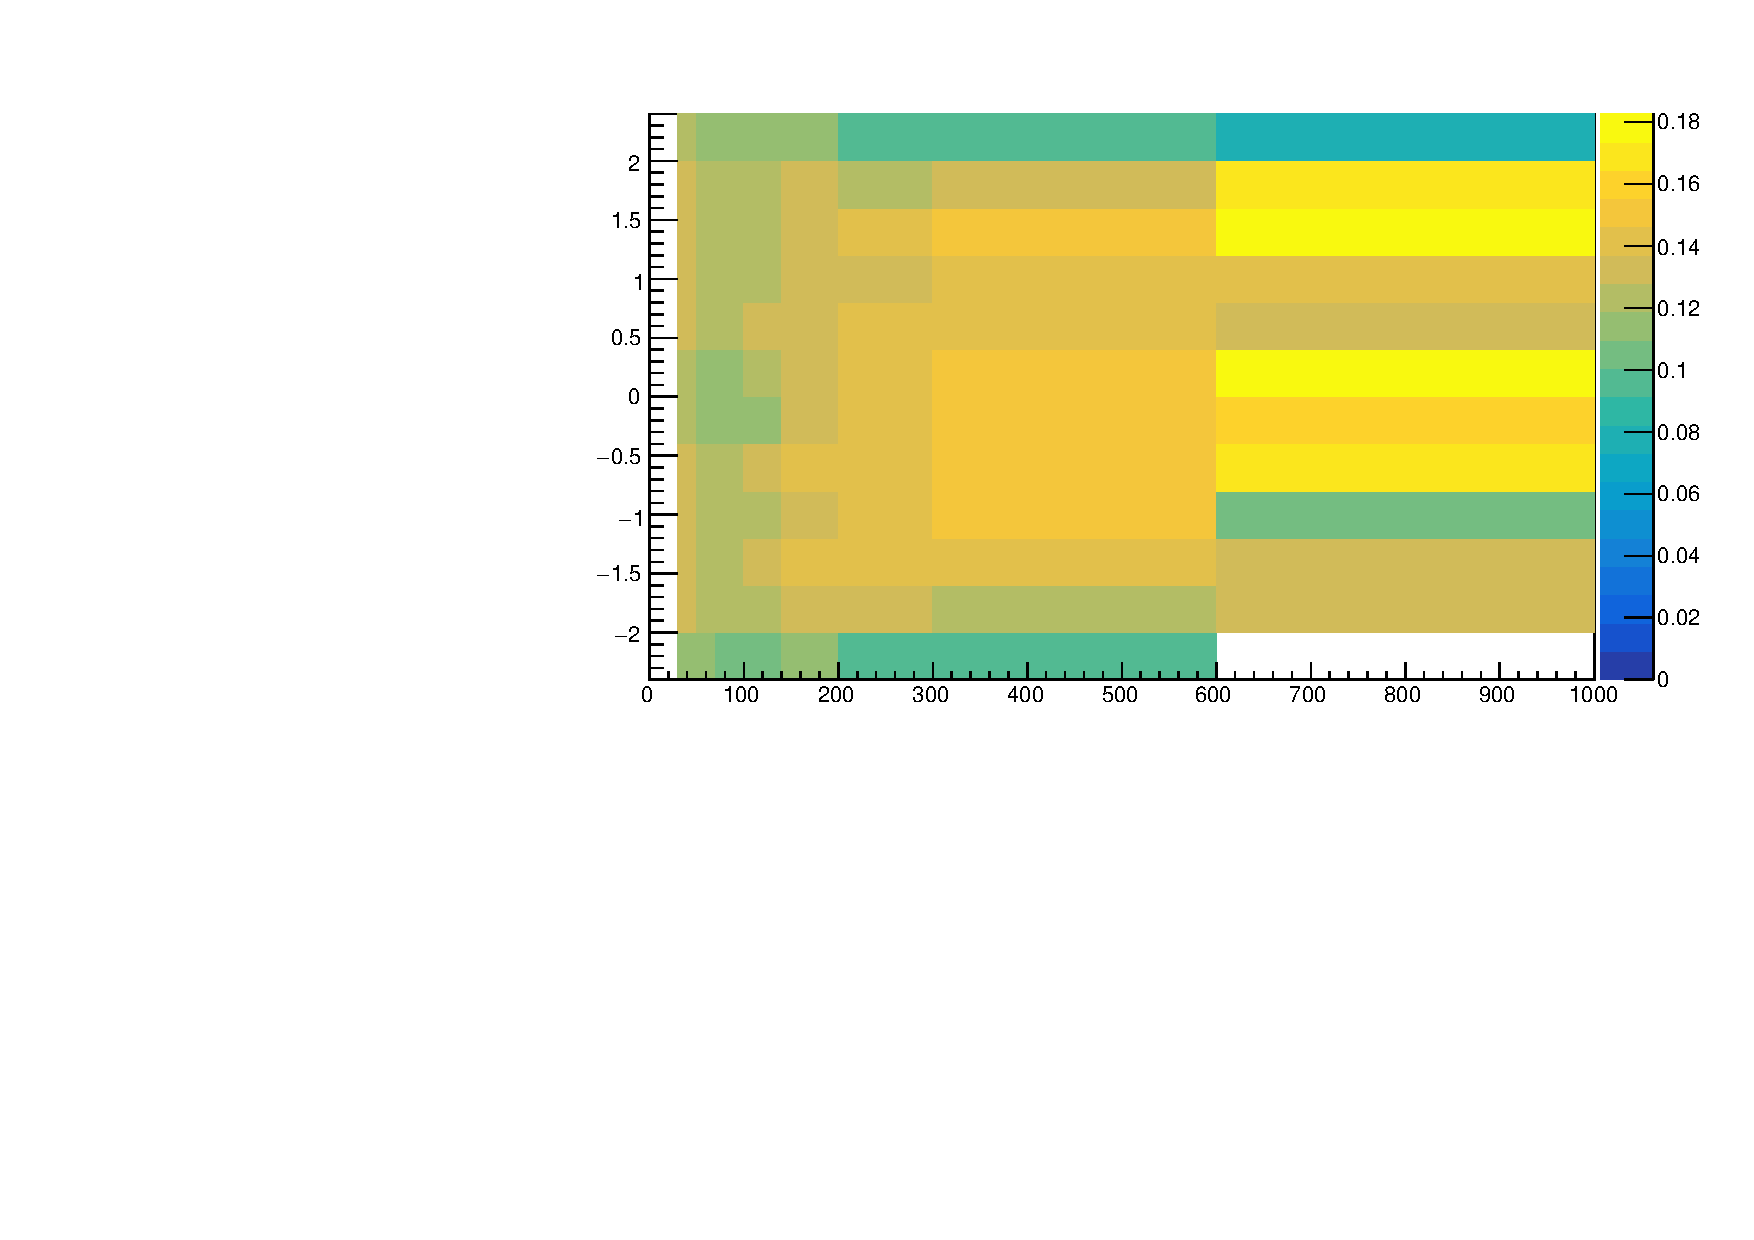
\includegraphics[width=0.45\textwidth]{Figures/DataMC/tt_eff_c.pdf}}\\
			    \subfigure[light(u,d,s,g)]{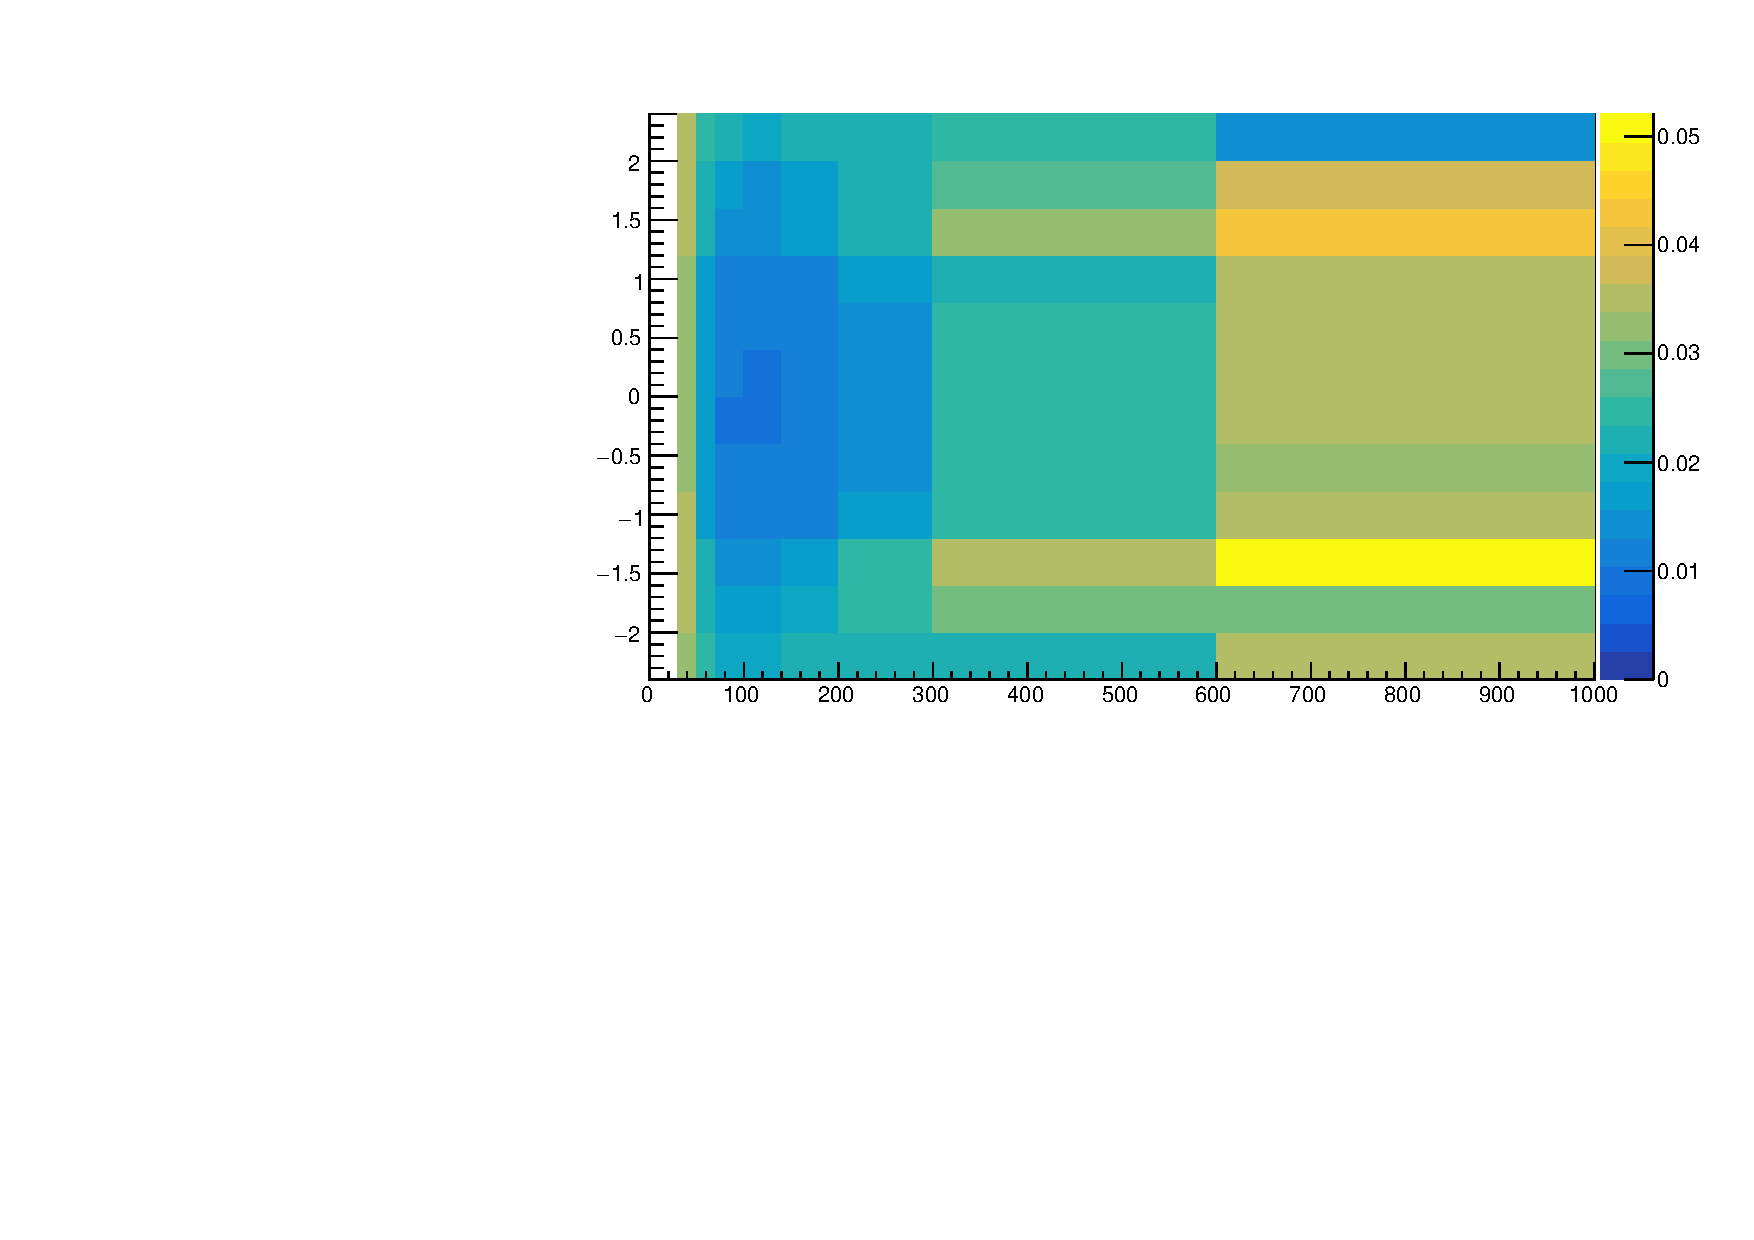
\includegraphics[width=0.45\textwidth]{Figures/DataMC/tt_eff_l.pdf}}
			   \caption{b-tagging efficiency of b, c, and light(udsg) flavor (x-axis:$p_T$, y-axis:$\eta$), under b-tagging working point Medium calculated by $t\bar{t}$ MC}
			\label{DataMC:fig:tt_eff_btag}
			\end{figure}
			\FloatBarrier


		\subsubsection{Weigh to Luminosity}
		\label{sssec:DataAndMC_lumi}




%%%--- TODO ---%%%
%%% table of the MC sample's Xsec and generated events number and generator -> weight to luminosity

\begin{center}
\begin{tabular}{ c c c c c }
\hline
Process sample & Cross Section (pb) & k-factor & Events Number & Generator \\ 
\hline
$t$$\bar{t}\rightarrow b \bar{b}jjl\nu$ & XXX & 1 & CCCCCC & AAAAAA \\
\hline
cell7 & cell8 & XXXXXX & cell7 & cell8 \\
\hline  {}
\end{tabular}
\end{center}


\FloatBarrier
